\documentclass{report}
\usepackage[utf8]{inputenc}
\usepackage[a4paper,margin=3cm,top=2cm]{geometry}
\usepackage{graphicx}
% graphics
\usepackage{tikz}
\usepackage{hyperref}
\usepackage{graphicx}
\usepackage{booktabs}
\usepackage{dirtree}
\usepackage{float}
\usepackage{tabularx}
\usepackage[indentafter]{titlesec}
\usepackage{xlop}
\usepackage{amsmath}
\usepackage{caption,subcaption}
\usepackage{fontawesome}
\usepackage{setspace}
%listings
\usepackage{xcolor}
\usepackage{listings}
\lstdefinestyle{verilog}{
	backgroundcolor=\color{gray!10!white},
	basicstyle=\footnotesize\ttfamily,
	breaklines=true,
	commentstyle=\color{gray},
	escapeinside={~}{~},
	frame=single,
	keywordstyle=\color{blue},
	language=verilog,
	numbers=left,
	numbersep=5pt,
	showstringspaces=false,   
	numberstyle=\tiny\color{gray},
	rulecolor=\color{gray},
	stringstyle=\color{purple},
	tabsize=4}
\lstnewenvironment{code}{\lstset{style=verilog}\latin}{\endlatin}

\lstdefinestyle{C}{
	backgroundcolor=\color{gray!10!white},
	basicstyle=\footnotesize\ttfamily,
	breaklines=true,
	commentstyle=\color{gray},
	escapeinside={~}{~},
	frame=single,
	keywordstyle=\color{blue},
	language=C,
	numbers=left,
	numbersep=5pt,
	showstringspaces=false,   
	numberstyle=\tiny\color{gray},
	rulecolor=\color{gray},
	stringstyle=\color{purple},
	tabsize=4}
\lstnewenvironment{ccode}{\lstset{style=C}\latin}{\endlatin}

\newcommand{\co}[1]{\lr{\lstset{style=verilog}\lstinline{#1}}}


\usepackage{fancyhdr}
\pagestyle{fancy}
\fancyhf{}
\fancyhead[LE,RO]{\leftmark}
\fancyhead[RE,LO]{بررسی الگوریتم‌های فشرده‌سازی و کاربردهای آن‌ها}
\fancyfoot[LE,RO]{\thepage}

\onehalfspacing
% persian
\usepackage[extrafootnotefeatures,localise]{xepersian}
\settextfont[
Scale = 1.2]{XB Zar}
\setlatintextfont[Scale=1.2,
 BoldFont={LiberationSerif-Bold.ttf}, 
 ItalicFont={LiberationSerif-Italic.ttf}]{LiberationSerif-Regular.ttf}
 
\begin{document}

\begin{titlepage}
\newcommand{\HRule}{\rule{\linewidth}{0.1mm}} 
\center % Center everything on the page

    
\includegraphics[scale=0.5]{figs/sharif.png}% \\[0.5cm] % 

    \vspace{0.2cm}
%---------------------------------------------------------------------------------
%	HEADING SECTIONS (Enter the Homework/assignment No., only)
%---------------------------------------------------------------------------------
    \textsc{ دانشگاه صنعتی شریف}\\[0.2cm] % heading course Number
    \textsc{ دانشکده مهندسی کامپیوتر}\\[0.2cm]% heading course Number
    % \textsc{\Large ارائهٔ مطالب علمی و فنی}\\[0.5cm] % heading course name

    % \textsc{\large مستند پروژه}\\[0.5cm] % Minor heading
%---------------------------------------------------------------------------------
%	TITLE SECTION (Replace 'TITLE' with the Homework/assignment Name/title)
%---------------------------------------------------------------------------------

\HRule \\[0.4cm]
    { \huge \bfseries بررسی الگوریتم‌های فشرده‌سازی \\و کاربردهای آن‌ها}\\[0.1cm] % Title of your Homework/assignment
\HRule \\[1.5cm]
 
%\maketitle
\begin{minipage}{0.4\textwidth}
\begin{center}

 \large
    
    \emph{نگارندگان:}\\
    محمد مهدی عرفانیان\\
    \vspace{1cm}
    
    \Large{ارائه مطالب علمی و فنی}\\[1cm]
    {دکتر همت‌یار}
    \end{center}
\end{minipage}
\vspace{30mm}

{\large \today}\\[1cm] % Date, change the \today to a set date if you want to be precise
\vfill % Fill the rest of the page with white-space
\end{titlepage}
\begin{abstract}

الگوریتم‌های فشرده‌سازی در طی عمر علوم کامپیوتر یکی از مهم‌ترین موضوعات مورد بحث آن بوده اند. در ابتدا با توجه
به کندی و ضعف سخت‌افزار و نیاز به انتقال حداقلی داده این الگوریتم‌ها مورد توجه قرار گرفتند؛ سپس با پیشرفت اینترنت و نیاز به
انتقال سریع داده، این الگوریتم‌ها دوباره به یکی از مهم‌ترین زمینه‌های تحقیق در علوم کامپیوتر تبدیل شدند، در این
زمان بسیاری از الگوریتم‌های مهم فشرده‌سازی داده کشف شدند. فرمت‌هایی هم‌چون mp3 یا 
jpeg 
- که از شناخته‌ترین فرمت‌های فشرده‌سازی حال حاضر هستند - ماحصل تحقیقات همین دوران اند. الگوریتم‌های فشرده‌سازی نه تنها راه خود را به مدیا
باز کردند بلکه در پردازش سیگنال نیز تاثیر عمده‌ای داشتند، تمامی ارتباطات رادیویی با استفاده از این الگوریتم‌ها سعی در 
بالا بردن امنیت و کاهش هزینه انتقال داده را دارند، در رمزنگاری نیز این الگوریتم‌ها راه‌گشایی می‌کنند و بسیاری از الگوریتم‌های رمز‌نگاری
و درهم‌سازی خود نوعی الگوریتم فشرده‌سازی محسوب می‌شوند. 

در این مستند سعی شده است تا مقدمه‌ای برای ورود به دنیای شگفت‌انگیز الگوریتم‌های فشرده‌سازی 
نوشته شود و خوانندگان را با تعاریف بنیادین و کاربردهای اصلی این الگوریتم‌ها آشنا کند، این مستند مقدمتاً دربارهٔ تعاریف اصلی و 
انواع الگوریتم‌های فشرده‌سازی و کاربردهای اصلی آن‌ها در دنیای امروز بحث می‌کند و پس از آن به بررسی جزیی‌تر دو فرمت 
اصلی فشرده‌سازی (
  mp3 و jpeg
) می‌پردازد. امید است تا مطالب این مستند مورد توجه خوانندگان عزیز قرار گیرد. 

به عنوان موخره چکیده باید نوشت که این مستند در راستای انجام پروژهٔ مستند‌سازی درس ارائه مطالب علمی و فنی تهیه شده است و 
برای سهولت کار استاد محترم درس برای تحصیل اطمینان از درستی مستندسازی و همچنین استفاده دانش‌جویان علاقه‌مند، سیر پیشرفت مستند به همراه کدهای
  	\LaTeX  \space
  در 
\textit{  \href{https://github.com/merfanian/DataCompressionDoc}{Github} 
}  قرار گرفته اند، لازم به ذکر است که این مستند به صورت متن‌باز ارائه شده و 
استفاده از آن بدون ذکر منبع برای همگان آزاد است. \\
  \vspace{10mm}

  
    \textbf{ کلمات کلیدی: الگوریتم‌های فشرده‌سازی، فشرده‌سازی  تصویر، فشرده‌سازی صوت، MP3، JPEG}
\end{abstract}
\tableofcontents
\listoffigures
\listoftables
\chapter{مقدمه}
\noindent
\textbf{
	\textit{
		توضیحی اولیه مبنی بر تعریف کلی فشرده‌سازی، انواع الگوریتم‌ها و کاربردها
	}
}
\pagenumbering{arabic}
\pagebreak
\section{تعریف}

الگوریتم‌های فشرده‌سازی، الگوریتم‌هایی هستند که می‌توان با استفاده از آن‌ها داده‌ها را طوری رمزنگاری کرد که در تعداد 	کمتری بیت نسبت به آرایش اولیه
قابل ارائه باشند\cite{data_compression}.
برای مثال می‌دانیم که برای ذخیرهٔ هر بیت اسکی
\efn{ASCII}
 هشت بیت فضا لازم است، می‌توان با استفاده از نگاشتی متشکل از حروف استفاده‌شده در 
یک متن تعداد بیت‌های مورد نیاز برای نشان دادن هر حرف استفاده‌شده در متن را کاهش داد.
با استفاده از این تکنیک در حقیقت متن را در قالب جدیدی فشرده کرده‌ایم.

\section{انواع الگوریتم‌های فشرده‌سازی}

در یک دسته‌بندی الگوریتم‌های فشرده‌سازی را به دو نوع زیر افراز می‌کنند.
\begin{itemize}
	\item  بدون هدررفت داده \efn{Lossless}
	\item  همراه هدررفت داده \efn{Lossy}
\end{itemize}

\subsection{الگوریتم‌های بدون هدررفت داده}
در این سری الگوریتم‌ها دادهٔ ورودی بدون هیچ‌گونه هدررفتی از دادهٔ خروجی قابل بازیابی‌ست، الگوریتم‌های 
این دسته با استفاده از افزونگی آماری تلاش می‌کنند تا نحوهٔ نمایش داده را در نگاشتی به نحوهٔ نمایش دیگری که به فضای کمتری نیاز دارد 
تبدیل کنند.
این الگوریتم‌ها در مواقعی که 
ثابت ماندن داده در طی فشرده‌سازی الزامی‌ست استفاده می‌شوند، همچنین معمولا برای بازیابی اطلاعات فشرده‌شده نیاز به 
داده‌هایی خارجی است که با کمک آن عمل بازیابی انجام می‌گیرد، از این رو می‌توان از این نوع الگوریتم‌ها در رمزنگاری نیز 
استفاده کرد. یکی از کاربردهای اصلی این الگوریتم‌ها در فشرده‌سازی متون است که اشتباه شدن حتی یک حر	ف می‌تواند باعث بدخوانی و 
بدفهمی متن اصلی گردد. الگوریتم‌های مشهور فشرده‌سازی بدون هدررفت داده به شرح زیر اند \cite{data_types}.

\begin{itemize}
	\item کدبندی طول اجرا\efn{\lr{Run-Length Enconding (RLE)}}
	\item فشرده‌سازی LZ\efn{\lr{Lempel-Ziv (LZ)}}
	\item کدگذاری هافمن\efn{\lr{Huffman Encoding}}
	\item تبدیل باروس-ویلر\efn{\lr{Burrows Wheeler Transform}}
\end{itemize}

البته لازم به ذکر است که در عمل از مجموعه‌ای از الگوریتم‌های فوق برای رسیدن به درصد مطلوب فشرده‌سازی استفاده می‌شود.
%todo: add my Compression project link to this section. 

\subsubsection{نمونه‌های الگوریتم‌های بدون هدررفت داده}
در عمل از الگوریتم‌های بدون هدررفت داده در مواقعی که 
پایداری داده‌های ذخیره‌شده حیاتی‌ست یا این که فایل در آینده به تعداد زیادی بار فشرده و گسترده می‌شود و از دست دادن قسمتی از داده در
هربار فشرده‌سازی منجر به اختلاف فاحش نهایی خواهد شد استفاده می‌شود. احتمالاً می‌توان مشهورترین فرمت فشرده‌سازی بدون هدررفت داده را
فرمت 
ZIP
نامید، این فرمت که برای فشرده‌سازی فایل‌های مختلف استفاده می‌شود به علت گستردگی استفاده در درون خود از 
الگوریتم‌های بدون هدررفت داده استفاده می‌کند، به جز فرمت ZIP 
فرمت‌های دیگری که استفاده‌های تخصصی‌تری دارند نیز از این الگوریتم‌ها استفاده می‌کنند که در ادامه به دو مورد مهم ایشان اشاره می‌کنیم.

\begin{itemize}
	\item \lr{PNG}\\
	در طراحی فرمت PNG برای فشرده‌سازی تصاویر از الگوریتم
	\lr{Lempel-Ziv-Welch (LZW)} 
	که الگوریتی Lossless است استفاده شده. 
	در 
	شکل 	\ref{example_1} و 
	جدول 	\ref{compare_1} 
	یک نمونه عکس در حالت فشرده‌نشده و فشرده‌شده با فرمت PNG
	و مقدار حجم آن در حالت‌های مختلف آورده شده است.

	\item \lr{FLAC \cite{flac}}\\
	کدک صوتی بدون هدررفت دادهٔ آزاد \efn{\lr{Free Lossless Audio Codec}} یا FLAC
	الگوریتمی که با استفاده از اطلاعات ذاتی داده‌های صوتی به فشرده‌سازی آن‌ها می‌پردازد، نرخ فشرده‌سازی این الگوریتم با توجه به 
	سطح فشرده‌سازی سازی آن معمولا بین ۴۰ تا ۶۰ درصد می‌باشد اما در حالت بیشینه ممکن است تا ۸۰ درصد هم برسد.
	
\end{itemize}

\begin{figure}[H]
	\centering
	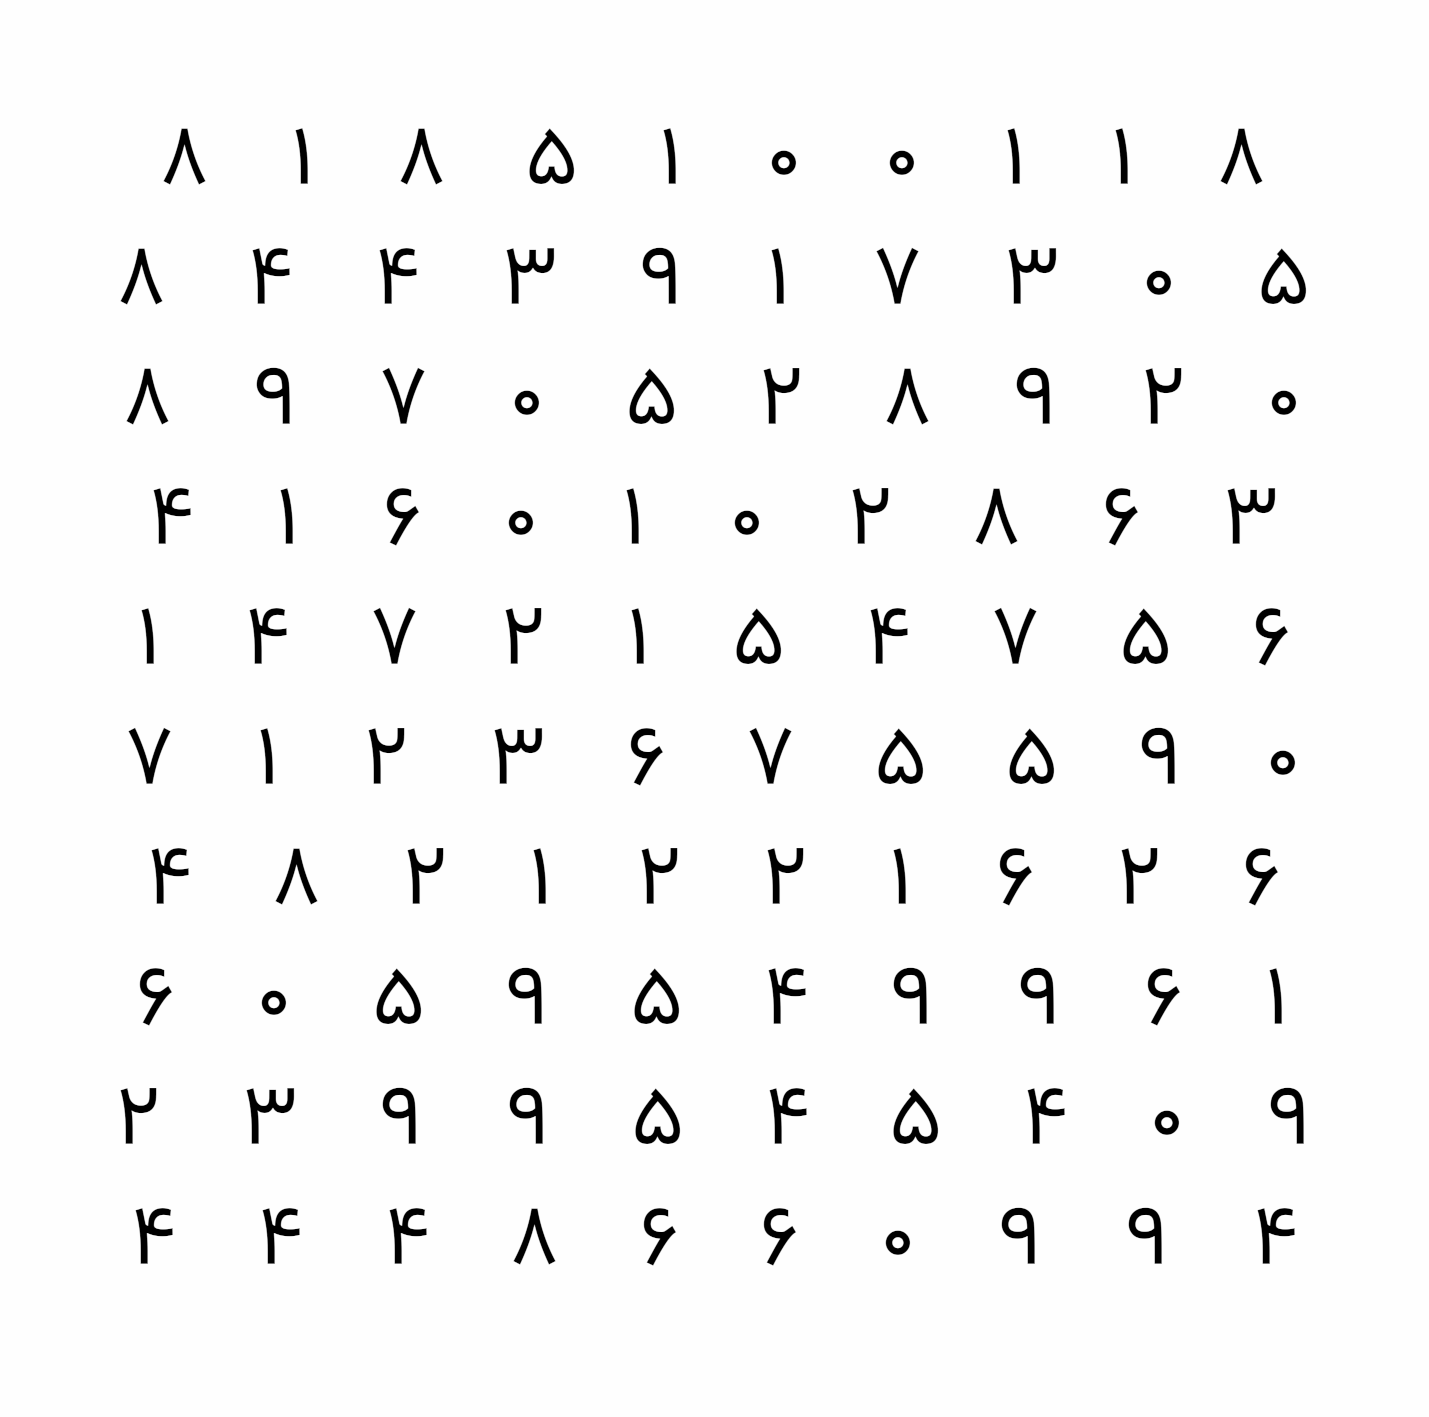
\includegraphics[scale=0.6]{figs/compressed.png}
	\caption[شکل نمونه برای تست میزان کمپرس در فرمت PNG ]{شکل نمونه برای تست میزان کمپرس در فرمت PNG \cite{my_picture}}
	\label{example_1}
\end{figure}

\begin{table}[H]
	\centering
	\caption{حجم فایل نمونه در فرمت PNG }
	\label{compare_1}
	\begin{tabular}{@{}ll@{}}
	\toprule
	Size & Format \\ \midrule
	7.7 مگابایت & BMP \\
	98 کیلوبایت & PNG \\ \bottomrule
	\end{tabular}
\end{table}



\subsection{الگوریتم‌های با هدررفت داده}

معمولا در فشرده‌سازی با هدررفت داده از تبدیل‌‌ فضایی 
\efn{\lr{Transformation}}
استفاده می‌شود که داده‌ها را از فضای حقیقی به فضایی دیگر(معمولا فرکانس) می‌برد و در آنجا از قسمت‌هایی از داده که تاثیرگذاری و حس‌پذیری کمتری
نسبت به دیگران دارند صرف نظر می‌شود، سپس وارون تبدیل اجرا شده و داده‌های کوچک‌شدهٔ جدید این بار با الگوریتم‌های 
بدون هدررفت داده فشرده می‌شوند. یکی از 
مشهورترین
تبدیل‌های فضایی
ها تبدیل کسینوسی گسسته
\efn{Discrete Cosine Transform (DCT)}
است که در فصل‌ دوم این مستند بیشتر با آن آشنا خواهیم شد
\cite{dct}.
\subsubsection{نمونه‌های الگوریتم‌های با هدررفت داده}
الگوریتم‌های با هدررفت داده با همه‌گیر شدن اینترنت و اشتراک‌گذاری 
بیشتر مدیا در فضای اینترنت بسیار گسترده شدند، از این رو اکثر این الگوریتم‌ها برای فشرده‌سازی فایل‌های صوتی-تصویری یا به اصطلاح 
مدیا\efn{Media}
استفاده می‌شوند. فرمت‌های زیر همگی در بطن خود از الگوریتم‌های با هدررفت داده برای فشرده‌سازی مدیا استفاده می‌کنند.

\begin{itemize}
	\item JPEG
	\item \lr{MP3}
	\item \lr{MP4}
	\item \lr{H.26x}
\end{itemize}
به عنوان نمونهٔ برای الگوریتم باهدررفت داده 
حالت فشرده‌شدهٔ عکس 
\ref{example_1}
با فرمت JPEG 
با کیفیت‌های مختلف در جدول 
\ref{compare_2}
آورده شده است.
% \footnote{در صورتی که تمایل به دیدن اصل فایل‌ها دارید می‌توانید به 
% \textit{  \href{https://github.com/merfanian/DataCompressionDoc/tree/master/LatexFiles/figs}{Github مستند} 
% } 
% مراجعه کنید.
% } 

\begin{table}[h]
	\centering
	\caption{حجم فایل نمونه در فرمت JPG}
	\label{compare_2}
	\begin{tabular}{@{}lll@{}}
	\toprule
	کیفیت(\%) & اندازه & فرمت \\ \midrule
	100 & 7.7 مگابایت & BMP \\
	100 & 98 کیلوبایت & PNG \\
	90 & 96.8 کیلوبایت & JPG \\
	50 & 62.9 کیلوبایت & JPG \\
	20 & 49  کیلوبایت& JPG \\ \bottomrule
	\end{tabular}
	\end{table}


\section{کاربردهای دیگر فشرده‌سازی}
الگوریتم‌های فشرده‌سازی داده علاوه بر این که در کاربرد اصلی خود یعنی فشرده کردن فایل‌ها بسیار استفاده می‌شوند اما کاربردهایی دیگری هم در دنیای
کامپیوتر دارند، به عنوان مثال یکی از حیاتی‌ترین عناصر پردازش سیگنال 
\efn{\lr{Signal Processing}} 
را فشرده‌سازی سیگنال تشکیل می‌دهد. در ارتباطات رادیویی برای بالا بردن امنیت و کم کردن هزینهٔ انتقال از فشرده‌سازی داده استفاده می‌شود. 

از دیگر کاربردهای جدید فشرده‌سازی داده ژنتیک است، رشته‌های دی‌ان‌ای
\efn{DNA}
و آر‌ان‌ای
\efn{RNA}
 را معمولا می‌توان به صورت
یک رشته متنی نشان داد و با الگوریتم‌های فعلی فشرده‌سازی متن فشرده کرد اما به دلیل این که این رشته‌ها طول و تعداد زیادی دارند
بهتر است از روش‌های دیگری برای بازیابی و فشرده‌سازی سریع آن‌ها استفاده کینم، با رشد سریع ژنتیک و بایوانفورماتیک در جهان و نیاز
مبرم به ذخیره‌سازی رشته‌های دی‌ان‌ای و آران‌ای 
الگوریتم‌های مختلفی مختص فشرده‌سازی این رشته‌ها معرفی شده اند\cite{dna}. 
\chapter{بررسی نحوهٔ فشرده‌سازی در فرمت JPEG}
\noindent
\textbf{
	\textit{
        توضیح نحوهٔ کار فشرده‌سازی در فرمت \lr{JPEG}، 
        مقدمه‌ای بر تبدیلی کسینوسی گسسته و 
        توضیح کلی کدگذاری هافمن
	}
}
\pagebreak

\section{تبدیل کسینوسی گسسته}

\subsection{
تعریف 
}

تبدیل کسینوسی گسسته\efn{\lr{Discrete cosine transform}} 
یا مختصراً
 DCT دنباله‌ای محدود از اعداد را به‌ صورت مجموع توابع کسینوسی با فرکانس‌های متفاوت نمایش می‌دهد

 
 تبدیل کسینوسی گسسته، شباهت بسیاری به تبدیل فوریه گسسته\efn{Discrete fourier transform} دارد، با این تفاوت که حاصل تبدیل فقط مقادیر حقیقی دارد بر خلاف تبدیل فوریه که منجر به مقادیر مختلط می شود.

 به صورت علمی‌تر می‌توان نوشت که 
 DCT 
 تابعی معکوس‌پذیر و خطی از 
 $R^N$ 
 به 
 $R^N$
 است.

 فرمول کلی DCT 
 برای فضای یک‌بعدی در معادله
 \ref{dct_eq} آمده
 است
\cite{dct}.
 \begin{equation}
 X_k = \sum_{n = 0}^{N - 1} x_n \cos [\pi / n  (n + 1/2)k]
 , k = 0, ..., N - 1
 \label{dct_eq}
 \end{equation}

 \section{تبدیل دنباله‌ای از پیکسل‌ها به تابع}
هر تصویر در حقیقت به صورت چهار ماتریس دوبعدی ذخیره می‌شود که هر ماتریس مقدار رنگی پیکسل را برای آن کانال رنگی
(
RBG و $\alpha$
)
نشان می‌دهد، برای فشرده کردن یک عکس ماتریس‌های کانال‌های رنگی مختلف را جداگانه فشرده می‌کنیم، کانال رنگی R 
را در نظر بگیرید، در این حالت یک ماتریس 
$n * m$ 
داریم که هر خانهٔ آن عددی بین ۰ تا ۲۵۵ را نشان می‌دهد، برای سادگی یک سطر از این ماتریس را در نظر بگیرید، این سطر معادل با یک 
آرایه از اعداد می‌باشد، در صورتی که تمامی اعداد را از دامنه ۰ تا ۲۵۵ به دامنه
$ -128 $ تا ۱۲۷ ببریم می‌توانیم این دنباله را با مجموعه‌ای از 
توابع کسینوسی بازتولید کنیم، این ضرایب همان ضرایبی‌ست که با استفاده از DCT 
می‌خواهیم به دست بیاوریم.

شکل
\ref{freq_1}
نمونه‌ای از توصیف عکس با توابع کسینوسی را نشان می‌دهد.

حال اگر دو تابع نشان‌داده شده در 
شکل 
\ref{freq_1}
را با هم جمع کرده و میانگین بگیریم، به نمایش فرکانس دیگری می‌رسیم که در شکل 
\ref{freq_2}
نشان داده شده است.
در صورتی که به شکل‌های متفاوت و با ضرایب متفاوت توابع مختلف کسینوسی را با هم جمع کنیم می‌توانیم هر فرکانسی را بسازیم. این کاری‌ست که در 
عمل الگوریتم 
DCT برای ما انجام می‌دهد.
\begin{figure}[]
        \centering
        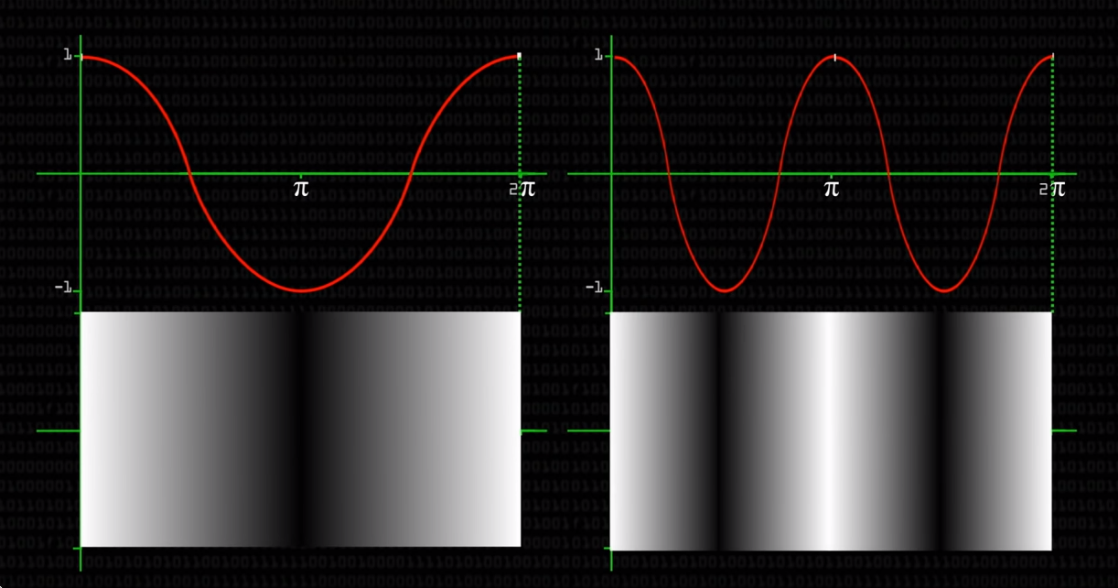
\includegraphics[width=\textwidth]{figs/freq_1.png}
        \caption[توصیف فرکانسی توابع 
        $\cos (x) , \cos (2x)$]{توصیف فرکانسی توابع 
        $\cos (x) , \cos (2x)$ \cite{youtube}}
        \label{freq_1}
\end{figure}

\begin{figure}[]
        \centering
        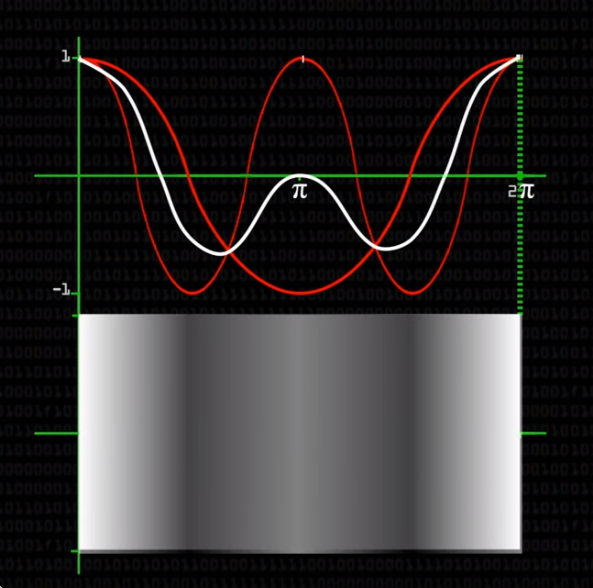
\includegraphics[width=0.5\textwidth]{figs/freq_2.png}
        \caption[توصیف فرکانسی تابع 
        $\cos (x) + \cos (2x) / 2$]{توصیف فرکانسی تابع 
        $\cos (x) + \cos (2x) / 2$ \cite{youtube}}
        \label{freq_2}
\end{figure}

\section{نحوهٔ کار JPEG}
برای فشرده‌سازی یک تصویر در JPEG 
مراحل زیر انجام می‌شود. 

\begin{itemize}
        \item تبدیل تصویر به بلوک‌های کوچک 
        \item تبدیل هر بلوک به مجموعه‌ای از توابع کسینوسی استاندارد با DCT
        \item تنظیم ضرایب متناسب برای بلوک‌های DCT 
        \item فشرده کردن ضرایب با استفاده از کدگذاری هافمن
\end{itemize}

\section{یک مثال از فشرده‌سازی JPEG}
برای درک بهتر مراحل گفته شده تلاش می‌کنیم تا ماتریس \ref{first_matrix} - که تصویر کانال خاکستری آن را در شکل 
\ref{jpeg_example}
مشاهده می‌شود -
را با الگوریتم‌های گفته‌شده فشرده‌سازی کنیم.
\begin{figure}[]
        \centering
        
\includegraphics[width=0.5\textwidth]{figs/jpeg_block.png}
        \caption[نمونهٔ تصویر برای فشرده‌سازی]{نمونهٔ تصویر برای فشرده‌سازی \cite{jpeg_example}}
        \label{jpeg_example}
\end{figure}
\begin{equation}      
        M = \begin{bmatrix}
                52 & 55 & 61 & 66 & 70 & 61 & 64 & 73\\
                63 & 59 & 55 & 90 & 109 & 85 & 69 & 72 \\
                62 & 59 & 68 & 113 & 144 & 104 & 66 & 73 \\
                63 & 58 & 71 & 122 & 154 & 106 & 70 & 60 \\
                67 & 61 & 68 & 104 & 126 & 88 & 68 & 70 \\
                79 & 65 & 60 & 70 & 77 & 68 & 58 & 75 \\
                85 & 71 & 64 & 59 & 55 & 61 & 65 & 83 \\
                87 & 79 & 69 & 68 & 65 & 76 & 78 & 94 

        \end{bmatrix}
        \label{first_matrix}
\end{equation}
هر عنصر ماتریس \ref{first_matrix} عددی بین ۰ تا ۲۵۵ دارد اما از آنجایی که تابع کسینوسی 
مقادیر بین $-1$ تا ۱ می‌گیرد نیازمندیم تا با کم کردن هر عنصر این ماتریس از 
۱۲۸ 
هر عنصر این ماتریس را به عددی بین $-128$ تا 127 تبدیل کنیم.
ماتریس   \ref{shifted_matrix} تبدیل‌شده است.
\begin{equation}    
                M^\prime = \begin{bmatrix}
                        -76 & -73 & -67 & -62 & -58 & -67 & -64 & -55\\
                        -65 & -69 & -73 & -38 & -19 & -43 & -59 & -56 \\
                        -66 & -69 & -60 & -15 & 16 & -24 & -62 & -55 \\
                        -65 & -70 & -57 & -6 & 26 & -22 & -58 & -59 \\
                        -61 & -67 & -60 & -24 & -2 & -40 & -60 & -58 \\
                        -49 & -63 & -68 & -58 & -51 & -60 & -70 & -53 \\
                        -43 & -57 & -64 & -69 & -73 & -67 & -63 & -45 \\
                        -41 & -49 & -59 & -60 & -63 & -52 & -50 & -34 
                        
                \end{bmatrix}
                \label{shifted_matrix}
\end{equation}

در گام بعدی مقادیر ماتریس تبدیل‌شده را با استفاده از الگوریتم 
DCT .به فضای فرکانس می‌بریم
هر مقدار از این ماتریس جدید برابر با ضریب فرکانس معادل در ماتریس 
استاندارد است. ماتریس \ref{transformed_matrix} ماتریس تبدیل‌شده‌ٔ ما خواهد بود.

\begin{equation}        
        F = \begin{bmatrix}
                -415.38 & -30.19 & -61.20 & 27.24 & 56.12 & -20.10 & -2.39 & 0.46\\
                4.47 & -21.28 & -60.76 & 10.25 & 13.15 & -7.09 & -8.54 & 4.88 \\
                -46.83 & 7.37 & 77.13 & -24.56 & -28.91 & 9.93 & 5.42 & -5.65 \\
                -48.53 & 12.07 & 34.10 & -14.76 & -10.24 & 6.30 & 1.83 & 1.95 \\
                12.12 & -6.55 & -13.20 & -3.95 & -1.87 & 1.75 & -2.79 & 3.14 \\
                -7.73 & 2.91 & 2.38 & -5.94 & -2.38 & 0.94 & 4.30 & 1.85 \\
                -1.03 & 0.18 & 0.42 & -2.42 & -0.88 & -3.02 & 4.12 & -0.66 \\
                -0.17 & 0.14 & -1.07 & -4.19 & -1.17 & -0.10 & 0.50 & 1.68 

        \end{bmatrix}
        \label{transformed_matrix}        
\end{equation}

هر کدام از عناصر ماتریس \ref{transformed_matrix} مقدار ضریب تاثیر فرکانس نشان‌داده‌شده در شکل 
\ref{freq_3} 
می‌باشند. 

\begin{figure}[]
        \centering
        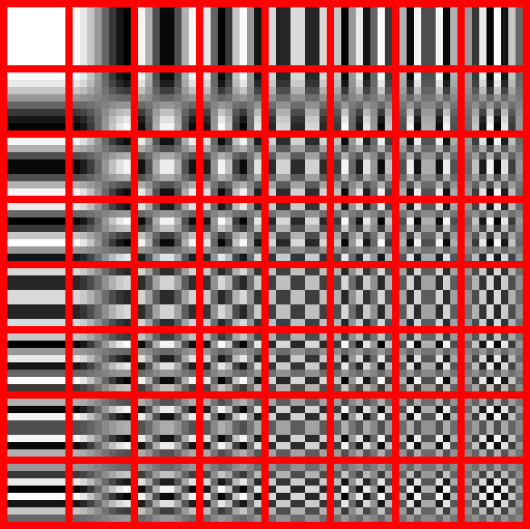
\includegraphics[]{figs/freq_3.png}
        \caption[ماتریس فرکانس‌های استاندارد]{ماتریس فرکانس‌های استاندارد \cite{standard_freqs}}
        \label{freq_3}
\end{figure}

تا به این لحظه هیچ مقداری از داده را برای فشره‌سازی از دست نداده‌ایم اما 
در این گام می‌خواهیم قسمت‌هایی از تصویر که برای چشم انسان قابل تشخیص نیستند
را حذف کنیم تا مقدار دادهٔ کمتری را ذخیره کنیم. 
باید توجه داشت که چشم انسان معمولا قادر به تشخیص و تمییز تصاویر با فرکانس‌های بالا در 
تصاویر نیست و همان‌طور که در ماتریس 
\ref{transformed_matrix}
هم مشاهده می‌شود ضریب این فرکانس‌ها نسبت 
به فرکانس‌های پایین بسیار کم است، می‌توانید به مقدار بسیار بزرگ ۴۱۵ برای
فرکانس بسیار پایین در راستای x و y در ماتریس توجه کنید تا 
این نکته روشن شود. حال باید ضرایب فعلی ماتریس را با تقریبی گرد کنیم و تاثیر 
فرکانس‌های بالا را کمتر از تاثیر فرکانس‌های پایین قرار دهیم، از این رو 
از جدولی به نام
جدول کوانتیزه کردن استفاده می‌کنیم. 

\subsection{جدول کوانتیزه کردن}
جدول کوانتیزه کردن\footnote{معادل فارسی برای 
\lr{Quantization} یافت نشد.}
جدولی است که در آن مقدار تاثیر هر فرکانس برای هر ردهٔ فشرده‌سازی 
برای عکس‌های JPEG به صورت جهانی استانداردسازی و تعیین شده‌است. 
برای مثال برای نرخ فشرده‌سازی ۵۰ درصد 
جدول کوانتیزه کردن در ماتریس 
\ref{quantization_table}
آمده است. این ماتریس برای کیفیت‌های مختلف فشرده‌سازی به صورت استانداردشده وجود دارد.
\begin{equation}      
        Q = \begin{bmatrix}
                16 & 11 & 10 & 16 & 24 & 40 & 51 & 61\\
                12 & 12 & 14 & 19 & 26 & 58 & 60 & 55 \\
                14 & 13 & 16 & 24 & 40 & 57 & 69 & 56 \\
                14 & 17 & 22 & 29 & 51 & 87 & 80 & 62 \\
                18 & 22 & 37 & 56 & 68 & 109 & 103 & 77 \\
                24 & 35 & 55 & 64 & 81 & 104 & 113 & 92 \\
                49 & 64 & 78 & 87 & 103 & 121 & 120 & 101 \\
                72 & 92 & 95 & 98 & 112 & 100 & 103 & 99 

        \end{bmatrix}
        \label{quantization_table}
\end{equation}

حال برای آخرین گام باید مقادیر ماتریس
\ref{transformed_matrix}
را بر مقادیر ماتریس 
\ref{quantization_table}
که همان ماتریس کوانتیزه کردن است
تقسیم کنیم و عدد به دست آمده را گرد کنیم. ماتریس نهایی برای فشرده‌سازی در ماتریس 
\ref{last_matrix}
آمده‌است.
\begin{equation}
       R = \begin{bmatrix}
                -26 & -3 & -6 & 2 & 2 & -1 & 0 & 0\\
                0 & -2 & -4 & 1 & 1 & 0 & 0 & 0 \\
                -3 & 1 & 5 & -1 & -1 & 0 & 0 & 0 \\
                -3 & 1 & 2 & -1 & 0 & 0 & 0 & 0 \\
                1 & 0 & 0 & 0 & 0 & 0 & 0 & 0 \\
                0 & 0 & 0 & 0 & 0 & 0 & 0 & 0 \\
                0 & 0 & 0 & 0 & 0 & 0 & 0 & 0 \\
                0 & 0 & 0 & 0 & 0 & 0 & 0 & 0 \\

        \end{bmatrix}
        \label{last_matrix}
\end{equation}

همان‌طور که در ماتریس 
\ref{last_matrix}
مشهود است تعداد بسیار زیادی از عناصر ماتریس جدید
مقدار صفر دارند (که بیشتر فرکانس‌های بالا را شامل می‌شوند)
در ادامهٔ فشرده‌سازی، ماتریس 
\ref{last_matrix}
به وسیلهٔ الگوریتم فشرده‌‌سازی بدون هدررفت دادهٔ
کدگذاری آنتروپی\efn{Entropy encoding} 
فشرده می‌شود و به همراه مقداری 
دادهٔ افزوده\efn{\lr{Meta data}}
مانند درصد فشرده‌سازی و داده‌های مورد نیاز برای بازیابی متن کدگذاری‌شده توسط کدگذاری آنتروپی ذخیره می‌شود. 
\section{کدگذاری آنتروپی}
کدگذاری آنتروپی نوعی کدگذاری تصاویر است که سعی می‌کند یک ماتریس را به صورت زیگزاگ به یک رشته متنی تبدیل کند و سپس با اجرای
الگوریتم کدگذاری طول اجرا و الگوریتم فشرده‌سازی هافمن این رشته را فشرده کند. شکل 
\ref{zigzag}
نحوهٔ تبدیل یک ماتریس عددی به یک رشتهٔ متنی در فشرده‌سازی آنتروپی رو نشان می‌دهد.

\begin{figure}[H]
        \centering
        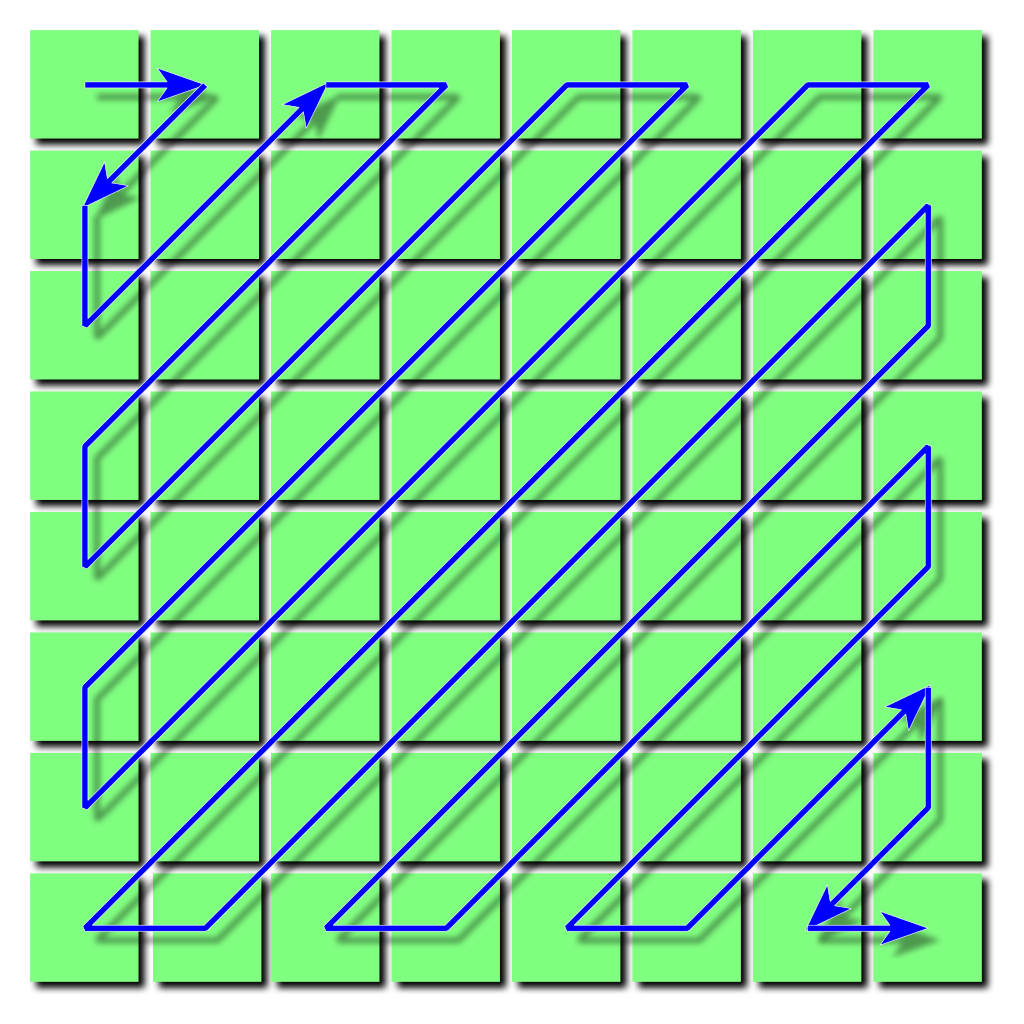
\includegraphics[width=0.5\textwidth]{figs/zigzag.png}
        \caption[کدگذاری زیگزاگ]{کدگذاری زیگزاگ \cite{zigzag}}
        \label{zigzag}
\end{figure}
در نتیجه دنبالهٔ زیگزاگی ماتریس \ref{last_matrix} به صورت زیر می‌شود. 

\begin{equation}
        -26, -3, 0, -3, -2, -6, 2, -4, 1, -3, 1, 1, 5, 1, 2, -1, 1, -1, 2, 0, 0, 0, 0, 0, -1, -1, 0 , \dots, 0
        \label{zigzag_string}
\end{equation}
در ادامه، این رشته یک بار با الگوریتم کدگذاری طول اجرا 
به یک رشتهٔ جدید کوتاه‌تر تبدیل می‌شود و سپس با الگوریتم هافمن فشرده می‌شود. 

\section{کدگذاری طول اجرا}
الگوریتم کدگذاری طول اجرا\efn{\lr{Run-length encoding}} یا RLE الگوریتمی‌ست که سعی می‌کند
به جای تکرار حروف تکراری پشت سر هم از اعداد برای نمایش تعداد آن‌ها استفاده کند. مثلا به جای رشتهٔ 
$aaa$
رشتهٔ 
$a3$ 
را قرار می‌دهد، در صورتی که حرف فقط یکبار تکرار شده باشد عدد ۱ نشان داده نمی‌شود. برای اجرای این کدگذاری بر روی 
رشتهٔ \ref{zigzag_string} صفرهای پایانی کدگذاری نمی‌شوند و برای هر عدد غیر صفر به جز عدد اول تعداد صفرهای قبل از آن
در رشته ذخیره می‌شود.
\section{فشرده‌سازی هافمن }
در انتها رشتهٔ خروجی الگوریتم کدگذاری طول اجرا با الگوریتم هافمن در سطح بیتی فشرده‌ می‌شود؛
در این قسمت مختصراً الگوریتم هافمن برای فشرده‌سازی یک رشتهٔ متنی شرح داده می‌شود.

\subsection{تعریف}
برای نمایش رشته در حالت 
اسکی\efn{ASCII}
برای هر حرف ۸ بیت فضا گرفته می‌شود و تمامی حروف با یک آرایهٔ هشت‌بیتی
نمایش داده می‌شوند. رشتهٔ زیر را در نظر بگیرید.
\begin{center}
        $S = bananasc$
\end{center}

برای نمایش این رشته در حالت اسکی به 
$ 8 * 8 = 64$ 
بیت فضا نیاز داریم، در صورتی که بخواهیم از طراحی 
با طول بیت ثابت برای هر حرف در این رشته استفاده کنیم می‌توانیم نظیرسازی 
جدول
\ref{huffman_fixed}
 را در نظر بگیریم. 

\begin{table}[H]
        \centering
        \caption{نوعی نظیرسازی حروف با طول ثابت برای هر حرف}
        \label{huffman_fixed}
        \begin{tabular}{ll}
        \hline
        نماد & حرف \\ \hline
        001 & a \\
        010 & b \\
        011 & n \\
        100 & s \\
        101 & c \\ \hline
        \end{tabular}
\end{table}

در این روش برای نشان دادن هر حرف به سه بیت فضا نیاز داریم پس در کل به
$ 8 * 3 = 24 $
بیت فضا نیاز است. 

اما در صورتی که به صورت دقیق‌تر به رشته نگاه کنیم متوجه می‌شویم که تعداد تکرار هر حرف
یکسان نیست و می‌توانیم برای نشان دادن هر حرف از تعداد بیت متغیر استفاده کنیم به شکلی که 
حروفی که بیشتر تکرار شده‌اند تعداد بیت کمتری بگیرند و حروفی که کمتر تکرار
شده اند از تعداد بیت بیشتری برای ذخیره‌‌سازی استفاده کنند. مثلا نظیرسازی جدول
\ref{huffman} 
را برای این رشته در نظر بگیرید.

\begin{table}[H]
        \centering
        \caption{نوعی نظیرسازی حروف با طول متغیر برای هر حرف}
        \label{huffman}
        \begin{tabular}{ll}
        \hline
        نماد & حرف \\ \hline
        0 & a \\
        110 & b \\
        10 & n \\
        1110 & s \\
        1111 & c \\ \hline
        \end{tabular}
\end{table}

درصورتی که رشتهٔ اصلی را با این نظیرسازی فشرده کنیم به بیت‌های زیر می‌رسیم.

\begin{center}
        $110010010011101111$
\end{center}

همان‌طور که در رشتهٔ جدید مشهود است تعداد بیت‌های استفاده‌شده برای نمایش
رشتهٔ اصلی به ۱۸ بیت کاهش پیدا کرده، نکته اساسی در این فشرده‌سازی 
این است که رشته به صورت یکتا قابل بازیابی باشد، در صورتی که به رشتهٔ بالا
دقت کنیم متوجه می‌شویم که تنها حالتی که می‌توان با توجه به حروف جدول برای
بازیابی بیت‌ها متصور شد همین حالتی‌ست که به رشتهٔ اصلی منجر می‌شود.
\begin{center}
        $110,0,10,0,10,0,1110,1111$ 
\end{center}

این اتفاق به این دلیل
رخ می‌دهد که شروع هیچ حرفی زیرمجموعهٔ پیشوندی هیچ رشتهٔ دیگری نیست، 
برای مثال در صورتی که حرف a با 
$0$ 
و حرف b
با 
$010$ 
و حرف 
n 
با 
$10$ 
نمایش داده می‌شدند برای رشتهٔ بیتی 
$010$
دو حالت
$an$
و 
$b$
می‌توانستیم متصور شویم، علت این اتفاق این است که رشتهٔ حرف 
a 
زیرمجموعهٔ حرف 
b
است. 

کلیت الگوریتم هافمن پیدا کردن بهترین کدگذاری برای هر حرف در رشتهٔ اصلی 
است که طول رشتهٔ نهایی کم‌ترین اندازه را داشته باشد و کدگذاری هیچ حرفی زیرمجموعهٔ پیشوندی حرف دیگری نشود، برای این کار از شبه کد زیر استفاده می‌شود \cite{huffman}.
\vspace{5mm}

\begin{code}
//Huffman Algorithm
n := |C|;
Q := C;
for i := 1 to n − 1 do
        allocate a new node z
        z.lef t := x := Extract-Min(Q);
        z.right := y := Extract-Min(Q);
        z.freq := x.freq + y.freq;
        Insert(Q, z);
end for
return Extract-Min(Q); {return the root of the tree}
\end{code}
\vspace{5mm}
شکل 
\ref{huffman_tree}
مراحل الگوریتم هافمن را برای یک رشته با تعداد تکرار در جدول
\ref{example_2}
نشان می‌دهد.


\begin{table}[H]
        \centering
        \caption{جدول تکرار حروف در یک رشته نمونه}
        \label{example_2}
        \begin{tabular}{ll}
        \hline
        تکرار & حرف \\ \hline
        5 & f \\
        9 & e \\
        12 & c \\
        13 & b \\
        d & 16 \\
        a & 45 \\ \hline
        \end{tabular}
\end{table}

\begin{figure}[H]
        \centering
        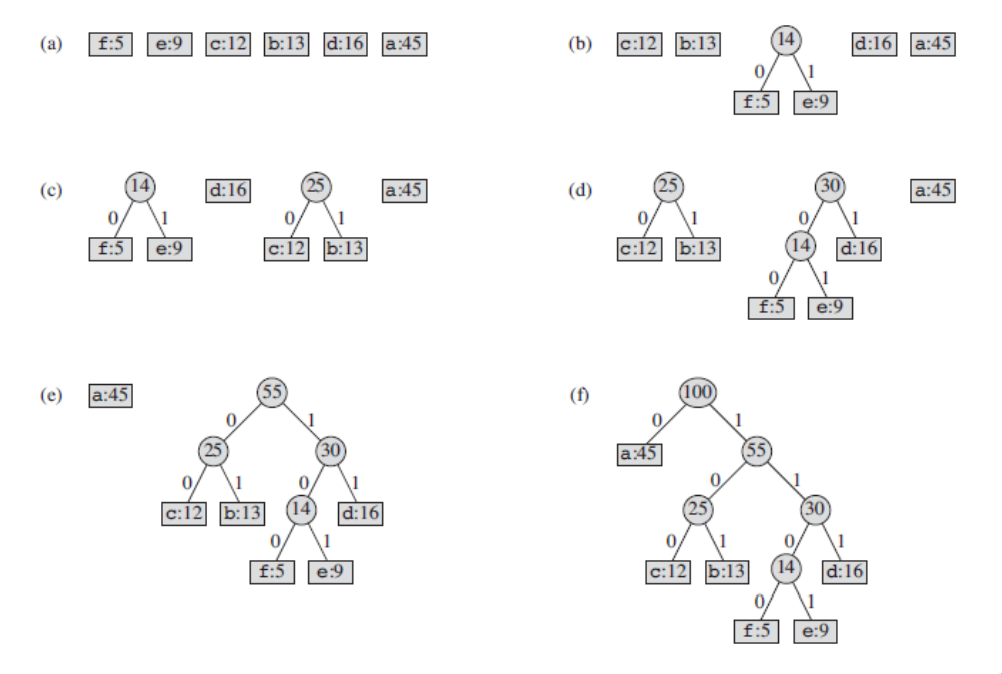
\includegraphics[width=\textwidth]{figs/huffamn_tree.png}
        \caption[مراحل الگوریتم هافمن]{مراحل الگوریتم هافمن \cite{huffman_tree}}
        \label{huffman_tree}
\end{figure}


\chapter{بررسی نحوهٔ فشرده‌سازی در فرمت \lr{MP3}}
\noindent
\textbf{
	\textit{
        توضیح نحوهٔ کار فشرده‌سازی در فرمت \lr{MP3}،
        تحلیل صدای انسان و توضیح کانال‌های فرکانسی
	}
}
\pagebreak

\section{ مقدمه}
در اواخر قرن بیستم و با شروع فراگیری اینترنت در جوامع مختلف، اشتراک‌گذاری 
فایل‌های رسانه‌ای مختلف مانند صوت، فیلم و تصویر در فضای اینترنت به یکی از خواست‌های همگانی و نیازهای اصلی مردم تبدیل شد اما 
مشکل اصلی در این میان، حجم زیاد فایل‌های رسانه‌ای و سرعت پایین انتقال داده در فضای اینترنت بود.
فرمت‌های فشرده‌سازی مختلفی برای حل این معضل پیشنهاد شدند که هر کدام با تکیه بر
تحلیل‌های آماری و یا حذف داده‌هایی غیرضروری در راستای کم کردن حجم فایل‌های رسانه‌ای می‌کوشیدند. در زمینهٔ  فشرده‌سازی فایل‌های
صوتی فرمت \lr{MP3} یقیناً فراگیرترین و موفق‌ترین فرمت به شمار می‌رود. در این فصل 
نگاهی کلی به نحوهٔ کار این فرمت و الگوریتم‌های با هدررفت داده به کاررفته در این فرمت خواهیم داشت. برای تقریب اذهان به بزرگی حجم فایل‌های صوتی فشرده‌نشده لازم به توجه است که هر
فایل صوتی در حالتی که هیچ مقداری از داده فشرده نشود در هرثانیه حدود ۱۷۶۰۰۰ بایت فضا می‌گیرد، یعنی یک صوت
یک دقیقه‌ای حدوداً به ۳۴ مگابایت فضا نیاز دارد \cite{uncompressed_source}.

\section{نرخ بیتی } 
برای درک بهتر مفاهیمی که در ادامهٔ متن با آن‌ها سر و کار داریم لازم است تا ابتدا با مفهوم نرخ بیتی \efn{bitrate} آشنا شویم، در مفاهیم علوم کامپیوتر، نرخ بیتی
معمولا  مقدار بیتی‌ست که در برای واحد زمانی ذخیره می‌شود \cite{bitrate_definition}، مثلاً وقتی نرخ بیتی یک موسیقی 
۳۲۰ کیلوبیت بر ثانیه
اعلام می‌شود به این معنی‌ست که برای هر ثانیه از این صوت ۳۲۰ کیلوبیت داده ذخیره شده است؛ همچنین نرخ بیتی می‌تواند سرعت انتقال داده در یک
کانال را بیان کند،‌ مثلاً در طراحی مودم‌های شبکه از این مفهوم برای نمایش سرعت انتقال داده استفاده می‌شود. 

\section{نحوهٔ کار \lr{MP3}}
تمرکز فرمت \lr{MP3} در فشرده‌سازی 
بر حذف اصواتی‌ست که توسط گوش انسان شنیده نمی‌شوند،‌ همان‌طور که از فصل دو به یاد دارید برای فشرده‌سازی تصاویر می‌توانستیم از بیت‌هایی که 
نمایان‌گر تصاویری با فرکانس بالا بودند صرف نظر کنیم زیرا توسط چشم انسان قابل تشخیص نبودند،‌ در فشرده‌سازی صوت نیز می‌توانیم 
 با مطالعهٔ ساختار شنوایی انسان اصواتی که به طور معمول توسط گوش انسان شنیده نمی‌شود را از صوت حذف می‌کنیم تا حجم فایل کاهش یابد.

 به شکل خلاصه می‌توان مراحل فشرده‌سازی در فرمت \lr{MP3} 
 را به شکل زیر خلاصه کرد \cite{how_mp3_works}.

 \begin{itemize}
         \item تبدیل صوت به قسمت‌های کوچک
         \item حذف صوت‌های خارج از محدودهٔ شنوایی انسان
         \item نمونه‌برداری از موسیقی با توجه به نرخ بیتی خواسته شده
         \item اضافه کردن افزونه‌ها و فشرده‌سازی نمونه
 \end{itemize}

\section{بررسی دستگاه شنوایی انسان}
برای فشرده‌سازی صوت باید در ابتدا اصواتی که توسط گوش انسان قابل شنیدن نیستند یا گوش انسان با جزییات کمتری آن‌ها را درک می‌کند را حذف کنیم، برای 
این کار به تحلیل صوت‌شناسی
\efn{Psychoacoustics}
نیاز داریم. 

نتایج تحلیل‌های صوت‌شناسی برای دستگاه شنوایی انسان موارد مفید زیر را اعلام می‌کند \cite{psychoacoustic}.

\begin{itemize}
        \item ضعف شنوایی بزرگسالان
        \item درک کمتر جزییات صداهای کم
        \item آستانهٔ شنوایی انسان
        \item اثر پوشش‌دهی صداهای بلند
\end{itemize}

به تفصیل موارد بالا و کاربرد‌های آنان در فشرده‌سازی را بررسی خواهیم کرد.

\subsection{ضعف شنوایی بزرگسالان}
در کودکی انسان‌ها معمولا می‌توانند اصواتی را که بین فرکانس‌های 0.1 تا ۲۰ کیلوهرتز باشند را بشنوند، اما با مسن شدن انسان معمولا حد بالای شنوایی 
به مقدار ۱۵ کیلوهرتز می‌رسد و در صورتی که به درصد فشرده‌سازی بالایی نیاز داشته باشیم می‌توانیم از فرکانس‌های بیش از ۱۵ کیلوهرتز صرف نظر کنیم.

\subsection{درک کمتر جزییات صداهای کم}
دستگاه شنوایی انسان معمولا به جزییات صداهای بلند بیش از صداهای آرام توجه می‌کند، در نتیجه می‌توانیم برای صداهایی که 
سطح فشار صوت \efn{\lr{Sound Pressure Level (db)}}
 کمتری دارند از نرخ بیتی پایین‌تری استفاده کنیم. 

 \subsection{آستانهٔ شنوایی انسان}
 گوش انسان برای هر فرکانس صوتی آستانهٔ شنوایی دارد که اگر سطح فشار صدا از آن کمتر باشد آن را نمی‌شنود، 
 شکل 
 \ref{human_hearing}
 این آستانه را برای فرکانس‌های مختلف نشان می‌دهد؛ در صورتی که سطح صوتی فرکانسی در هر قسمت از مقدار آستانهٔ آن کمتر باشد آن صدا شنیده نمی‌شود و 
 می‌توان آن را حذف کرد.

 \begin{figure}[]
         \centering
         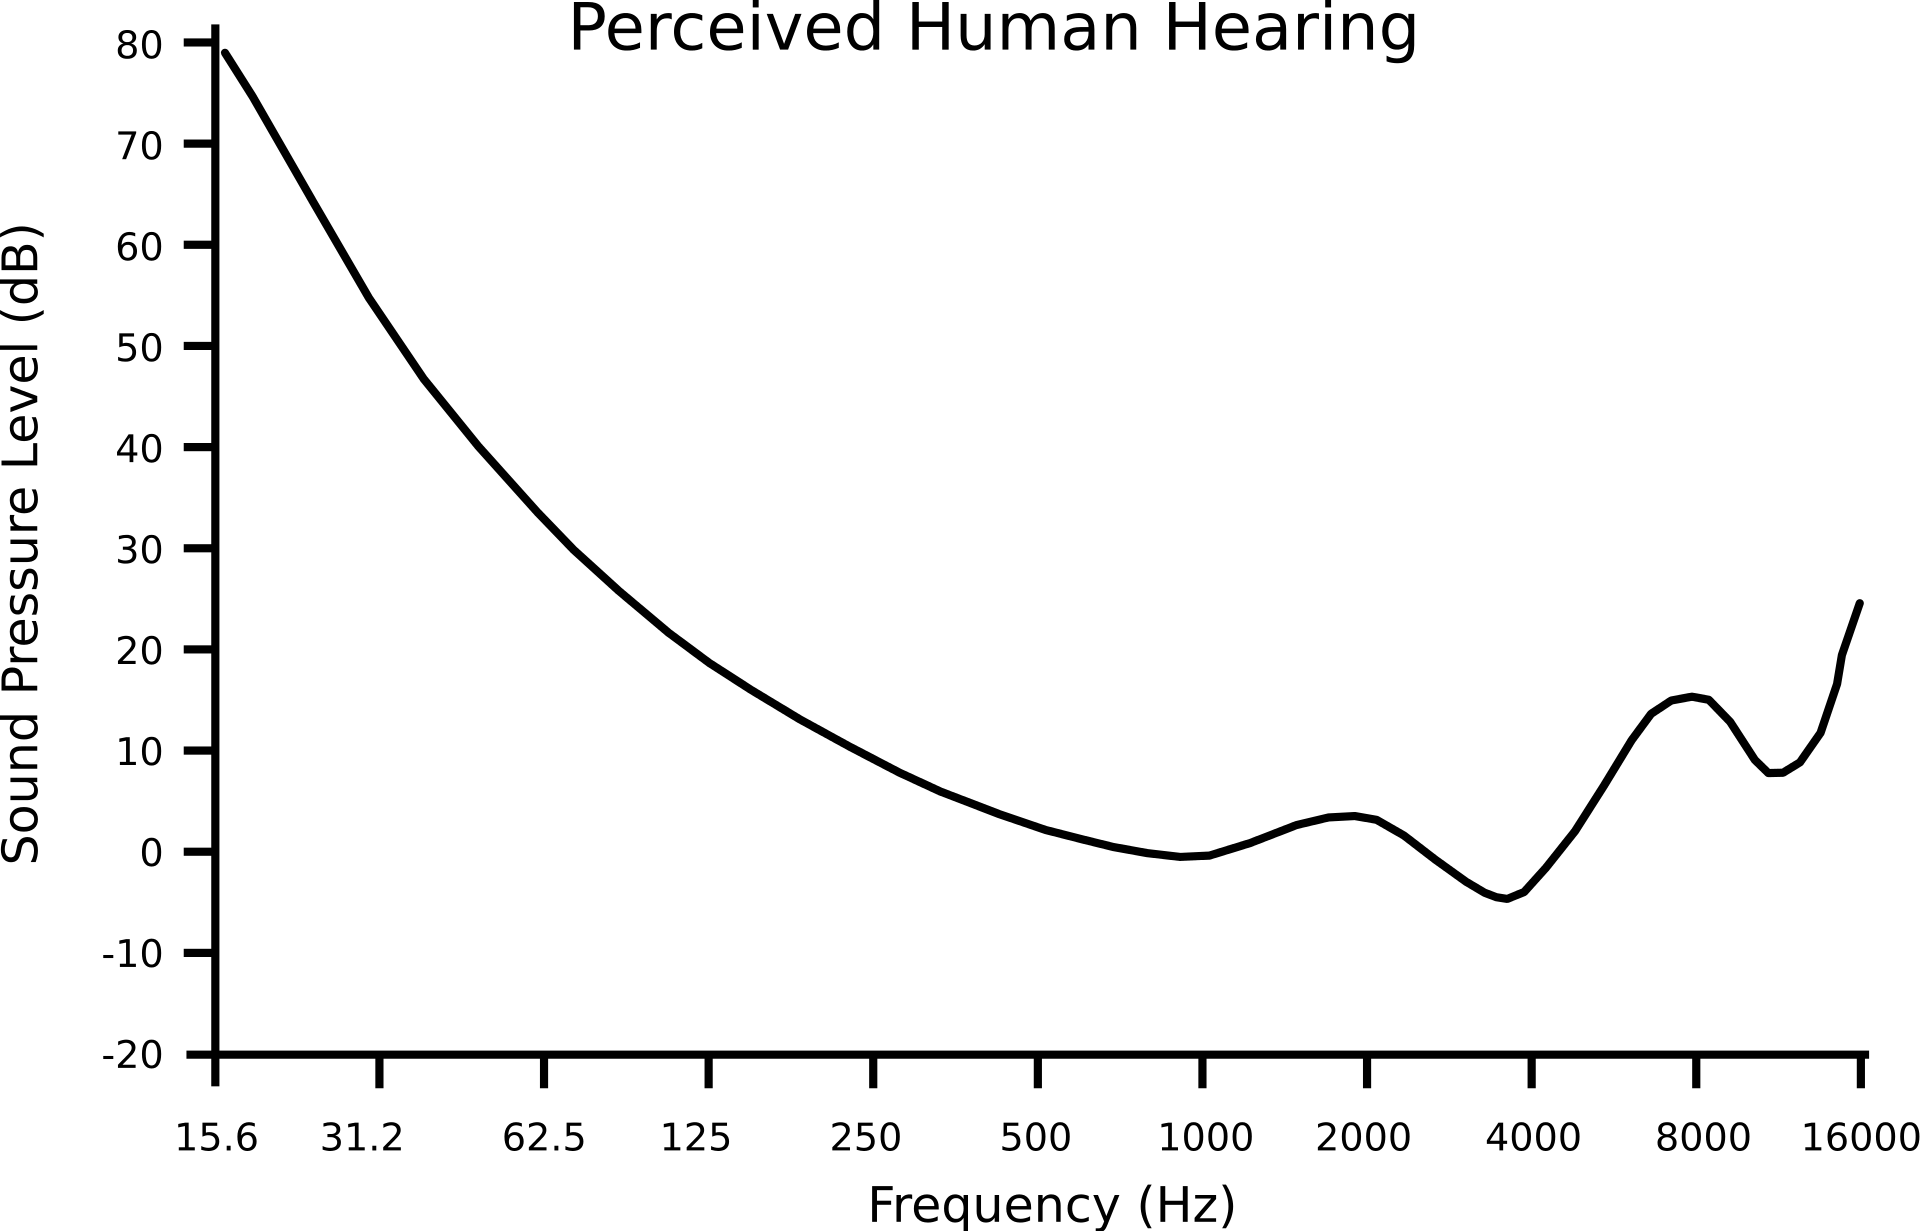
\includegraphics[width=\textwidth]{figs/human_hearing.png}
         \caption[آستانهٔ شنوایی انسان برای فرکانس‌های مختلف]{آستانهٔ شنوایی انسان برای فرکانس‌های مختلف \cite{percieved_human_hearing}}
         \label{human_hearing}
 \end{figure}
 \subsection{اثر پوشش‌دهی صداهای بلند}
 هنگامی که در یک محدودهٔ فرکانسی یک صدای بلند رخ دهد گوش انسان نمی‌تواند صداهای آرام با فرکانس‌های نزدیک به آن را تشخیص دهد و بشنود
 حتی اگر سطح صوتی آن از آستانهٔ شنوایی انسان بیشتر باشد، به این اثر در گوش انسان اثر پوشش‌دهی 
 \efn{\lr{Masking Effect}} 
 گفته می‌شود. 
 مثالی از اثر پوشش‌دهی در شکل 
 \ref{masking_effect}
 نشان داده شده است. 

 \begin{figure}[]
         \centering
         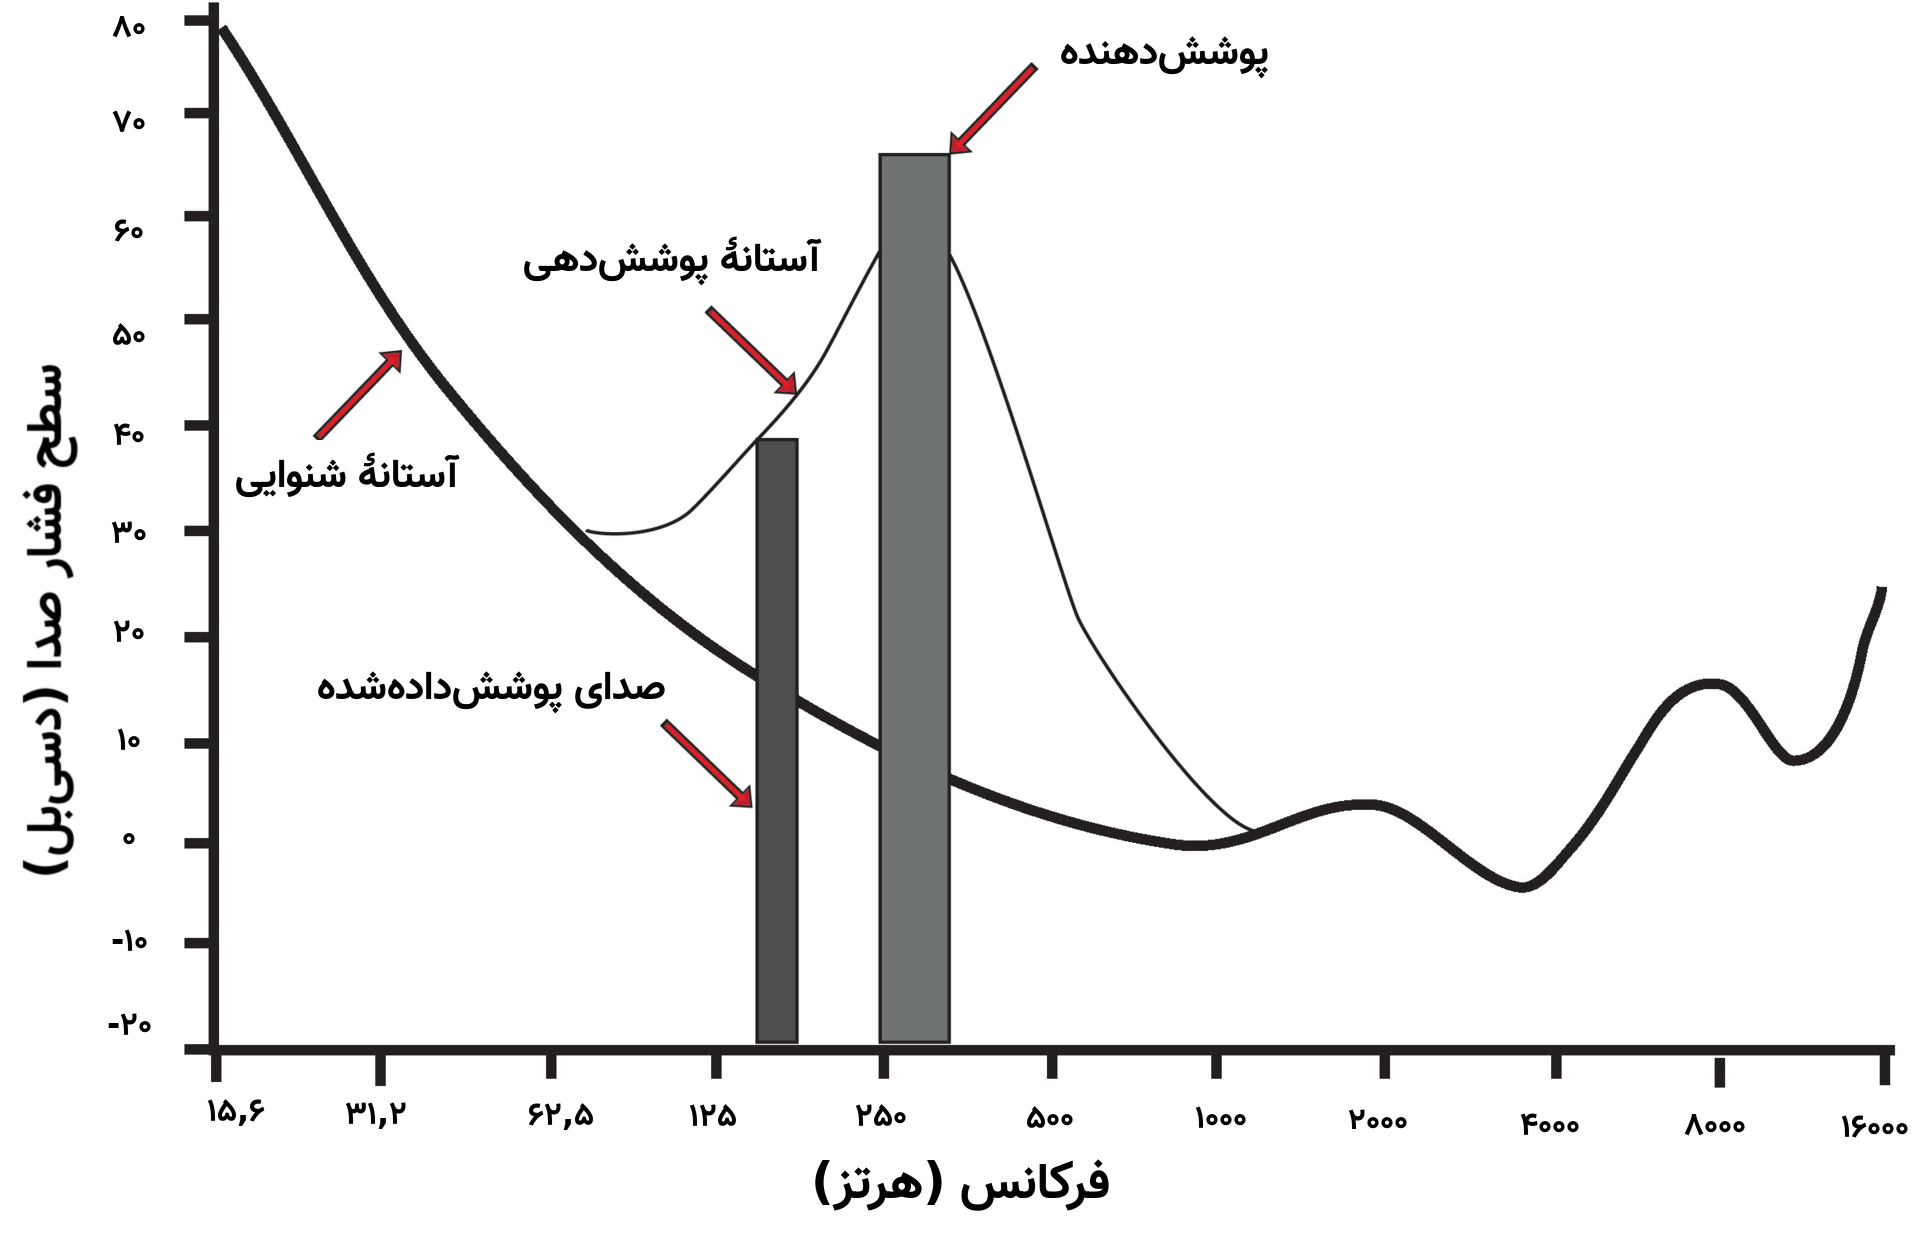
\includegraphics[width=\textwidth]{figs/masking_effect.png}
         \caption[اثر پوشش‌دهی صدا]{اثر پوشش‌دهی صدا \cite{audio_masking}}
         \label{masking_effect}
 \end{figure}

 \section{فشرده‌سازی \lr{MP3} در عمل}

 پس از بررسی انتزاعی اتفاقاتی که برای فشرده‌سازی در فرمت \lr{MP3} میافتد نیازمند آنیم تا 
 با یک مثال جزییات فنی پیاده‌سازی این فرمت را نیز بررسی کنیم. 

 هنگامی که یک صوت برای فشرده‌ شدن انتخاب می‌شود ابتدا به تکه‌های صوتی کوچک‌تر تقسیم می‌شود و با تبدیل کسینوسی گسسته که در فصل 
 دوم معرفی شد به فضای فرکانس برده می‌شود، پس از آن اصواتی که فرکانس‌هایی پایین‌تر از آستانهٔ شنوایی انسان دارند حذف می‌شوند و همین‌طور برای
 هر کانال صوتی عامل پوشش‌دهنده \efn{Masker}  و عوامل پوشش‌پذیر \efn{Maskee}
 شناسایی می‌شوند و بیت‌های مربوط به عوامل پوشش‌پذیر حذف می‌شوند، همچنین برای صداهای بلند مقداری از جزییات اصوات آرام‌تر را حذف می‌کنیم زیرا
 توسط ذهن انسان تشخیص داده نمی‌شوند. 

  پس از این تغییرات دوباره به فضای زمان برمی‌گردیم تا نمونه‌گیری را با توجه به 
 نرخ بیتی خواسته‌شده انجام دهیم؛ دقت کنید که تا این‌جای کار هیچ مقداری از بیت‌هایی که توسط دستگاه شنیداری انسان قابل شنیدن باشند از دست نرفته‌اند.

 در گام سوم با توجه به نرخ بیتی از هر قسمت کوچک ساخته شده نمونه برداری می‌کنیم و سپس به گام آخر فشرده‌سازی می‌رسیم
 در این گام اطلاعاتی که برای بازیابی هر قسمت مورد نیاز است به همراه تعدادی بیت که برای تشخیص خطا قرار می‌گیرند را در سرتیتر\efn{Header}
 هر قسمت قرار می‌دهیم و سپس داده اصلی را قرار می‌دهیم. مختصرا می‌توان گفت که هر بلوک داده موارد زیر را در خود دارد. 

 
 \begin{itemize}
        \item سرتیتر
        \begin{multicols}{2}
                \begin{itemize}
                        \item کد همگام‌سازی\efn{\lr{Sync word}}
                        \item نسخه\efn{\lr{Version}}
                        \item لایه صوتی\efn{\lr{Layer}}
                        \item بیت جلوگیری از خطا\efn{\lr{Error protection bit}}
                        \item نرخ بیتی\efn{\lr{Bitrate}}
                        \item فرکانس
                        \item بیت فاصله\efn{\lr{Padding bit}}
                        \item بیت خصوصی\efn{\lr{Private bit}}
                        \item حالت صوت\efn{Mode}
                        \item دادهٔ کپی‌شده\efn{Copy}
                        \item دادهٔ اصلی\efn{Original}
                        \item بیت تاکید\efn{Emphasis}
                \end{itemize}
        \end{multicols}
                \item داده صوتی
 \end{itemize}


\end{document}
